\documentclass[../main.tex]{subfiles}

\clearpage

\section{Menús} \label{section:app-menu}

\subsection{Menú de Fichero} \label{subsection:app-fich}

\begin{figure}[H]
    \centering
    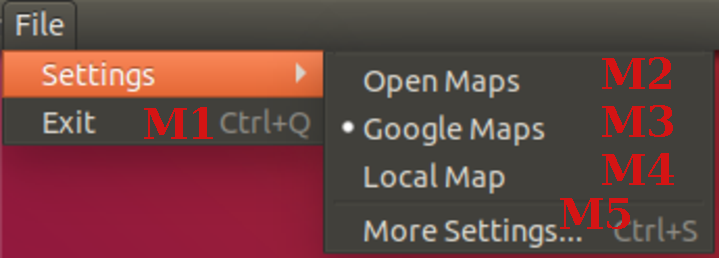
\includegraphics[width=0.5\textwidth]{man/menu.pdf}
\end{figure}

\begin{table}[H]
    \centering
    \begin{threeparttable}
        \begin{tabular}{| l | l |}
            \hline
            \thead{Nº} & \thead{Descripción} \\ \hline
            
            M1 & Opción para cerrar la aplicación. \\ \hline
            M2 & Opción de cambio de escena a mapas abiertos. \\ \hline
            M3 & Opción de cambio de escena a mapas de Google. \\ \hline
            M4 & Opción de cambio de escena a mapas locales. \\ \hline
            M5 & Opción para abrir ventana de configuración (Ver \ref{subsection:app-config}). \\ \hline
        \end{tabular}
        
    \end{threeparttable}
\end{table}

\clearpage

\section{Ventana Principal} \label{section:app-vent-princ}

\subsection{Panel de Navegación} \label{subsection:app-naveg}

\begin{figure}[H]
    \centering
    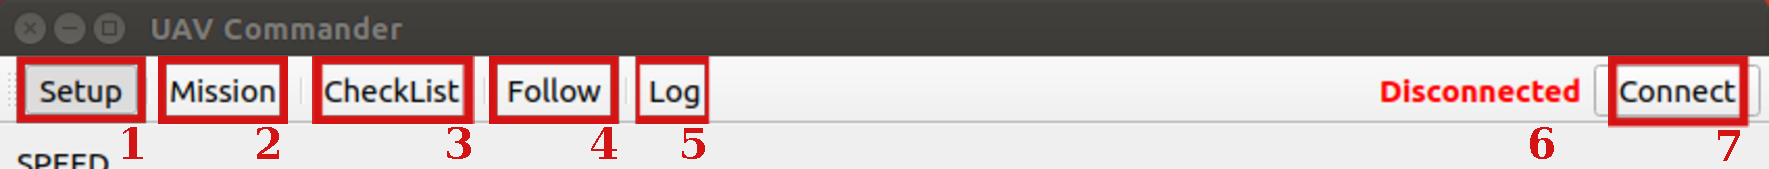
\includegraphics[width=\textwidth]{man/navegacion.pdf}
\end{figure}

\begin{table}[H]
    \centering
    \begin{threeparttable}
        \begin{tabular}{| l | l |}
            \hline
            \thead{Nº} & \thead{Descripción} \\ \hline
            
            1 & Botón para acceder a la pestaña \emph{Setup} (Ver \ref{subsection:app-setup}). \\ \hline
            2 & Botón para acceder a la pestaña \emph{Mission} (Ver \ref{subsection:app-mission}). \\ \hline
            3 & Botón para acceder a la pestaña \emph{Checklist} (Ver \ref{subsection:app-check}). \\ \hline
            4 & Botón para acceder a la pestaña \emph{Follow} (Ver \ref{subsection:app-follow}). \\ \hline
            5 & Botón para acceder a la pestaña \emph{Log} (Ver \ref{subsection:app-log}). \\ \hline
            6 & Etiqueta que muestra el estado de la conexión. \\ \hline
            7 & Botón para establecer/cortar la conexión. \\ \hline
        \end{tabular}
        
    \end{threeparttable}
\end{table}

\clearpage

\subsection{Pestaña \emph{Setup}} \label{subsection:app-setup}

\begin{figure}[H]
    \centering
    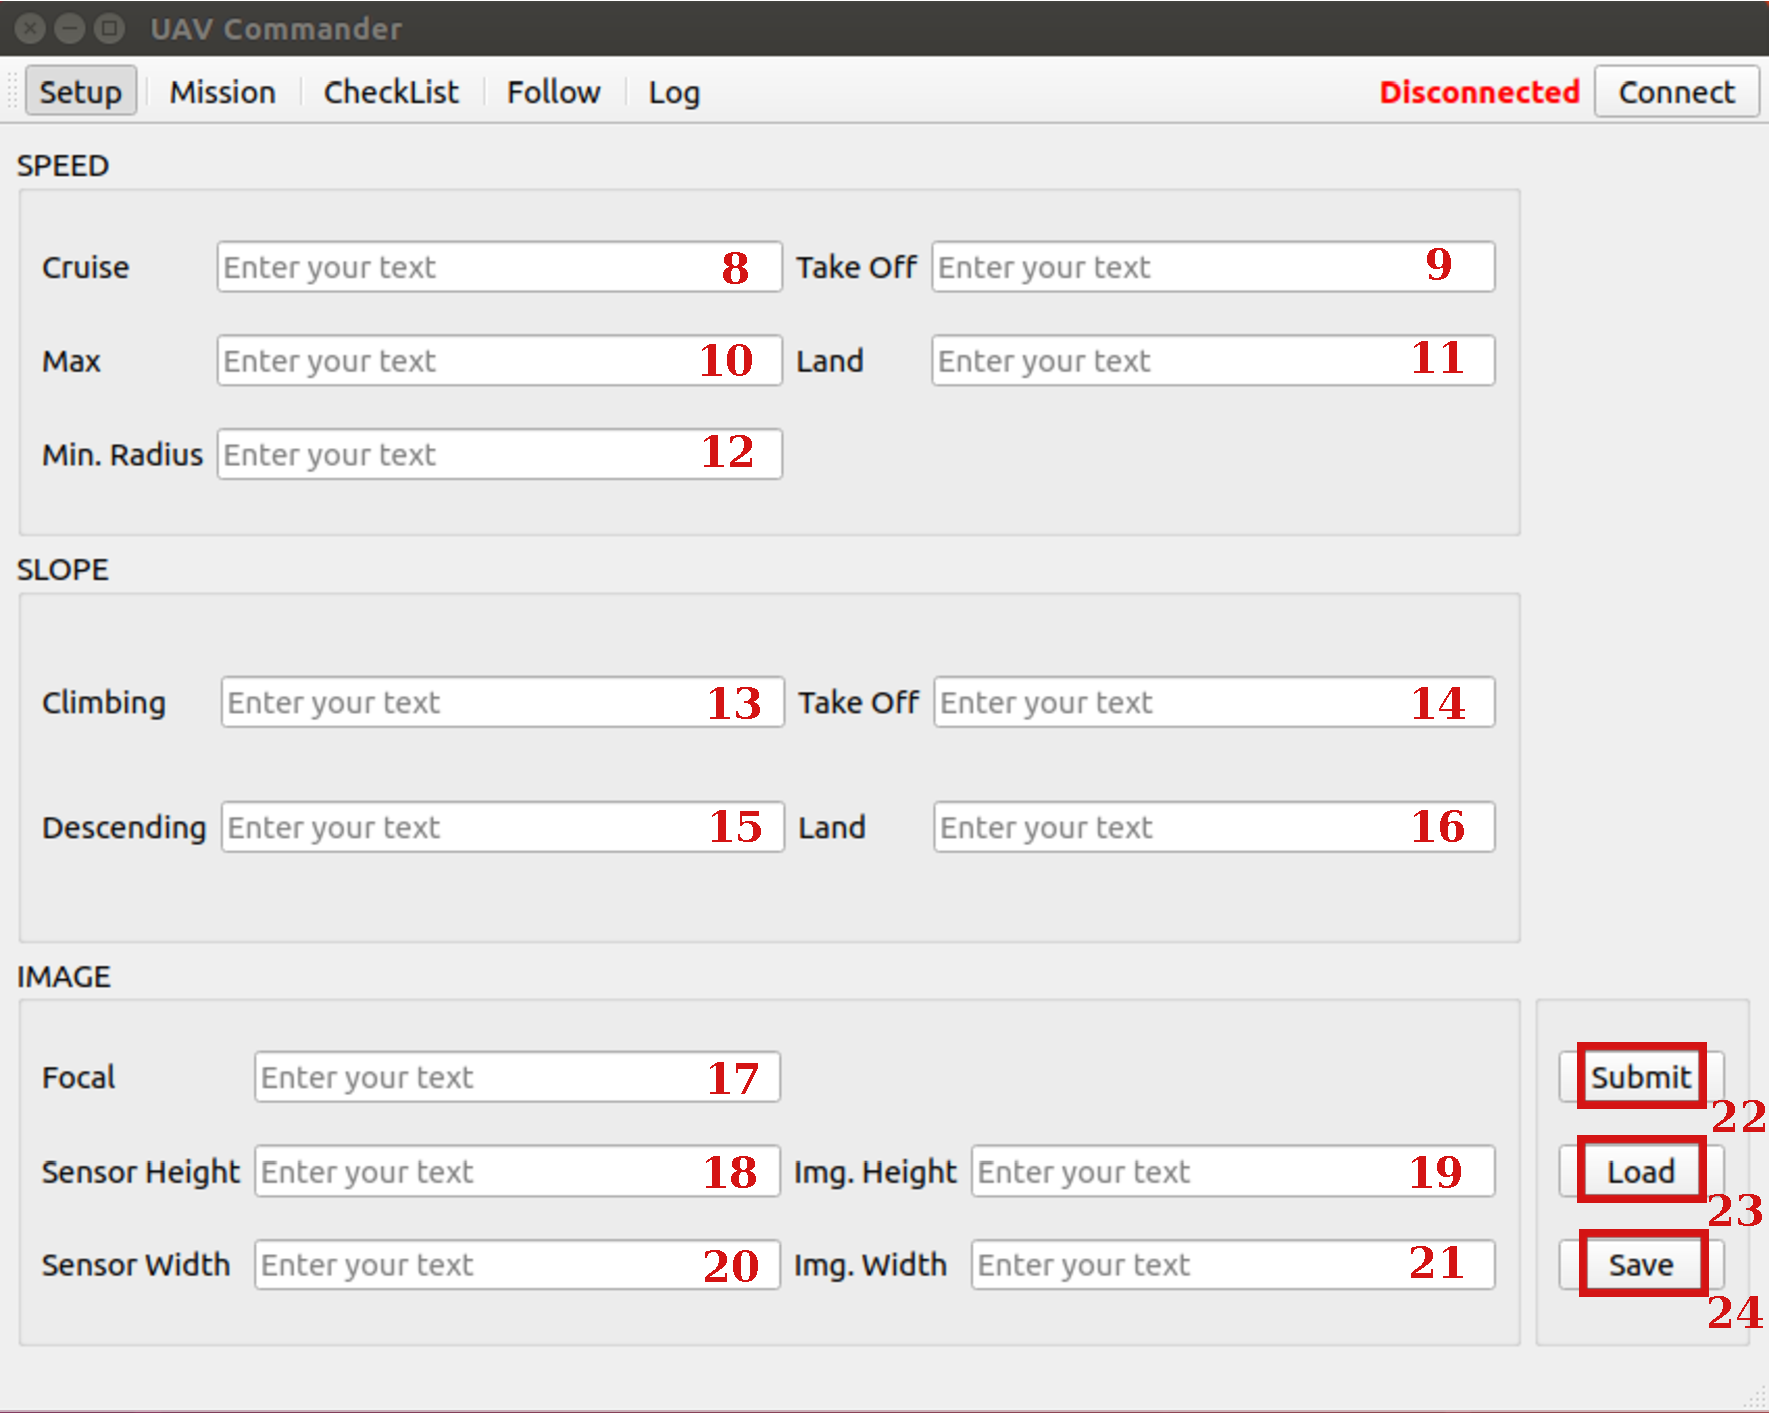
\includegraphics[width=\textwidth]{man/setup.pdf}
\end{figure}

\begin{table}[H]
    \centering
    \begin{threeparttable}
        \begin{tabular}{| l | l |}
            \hline
            \thead{Nº} & \thead{Descripción} \\ \hline
            
            8  & Velocidad de crucero (m/s). \\ \hline
            9  & Velocidad de despegue (m/s). \\ \hline
            10 & Velocidad máxima (m/s). \\ \hline
            11 & Velocidad de aterrizaje (m/s). \\ \hline
            12 & Radio mínimo de giro (m). \\ \hline
            13 & Pendiente de ascenso (º). \\ \hline
            14 & Pendiente de despegue (º). \\ \hline
            15 & Pendiente de descenso (º). \\ \hline
            16 & Pendiente de aterrizaje (º). \\ \hline
            17 & Distancia focal del sensor (mm). \\ \hline
            18 & Alto del sensor (mm). \\ \hline
            19 & Alto de la imagen (px). \\ \hline
            20 & Ancho del sensor (mm). \\ \hline
            21 & Ancho de la imagen (px). \\ \hline
            22 & Botón crear la configuración. \\ \hline
            23 & Botón para cargar una configuración. \\ \hline
            24 & Botón para guardar la configuración. \\ \hline
        \end{tabular}
        
    \end{threeparttable}
\end{table}

\clearpage

\subsection{Pestaña \emph{Mission}} \label{subsection:app-mission}

\begin{figure}[H]
    \centering
    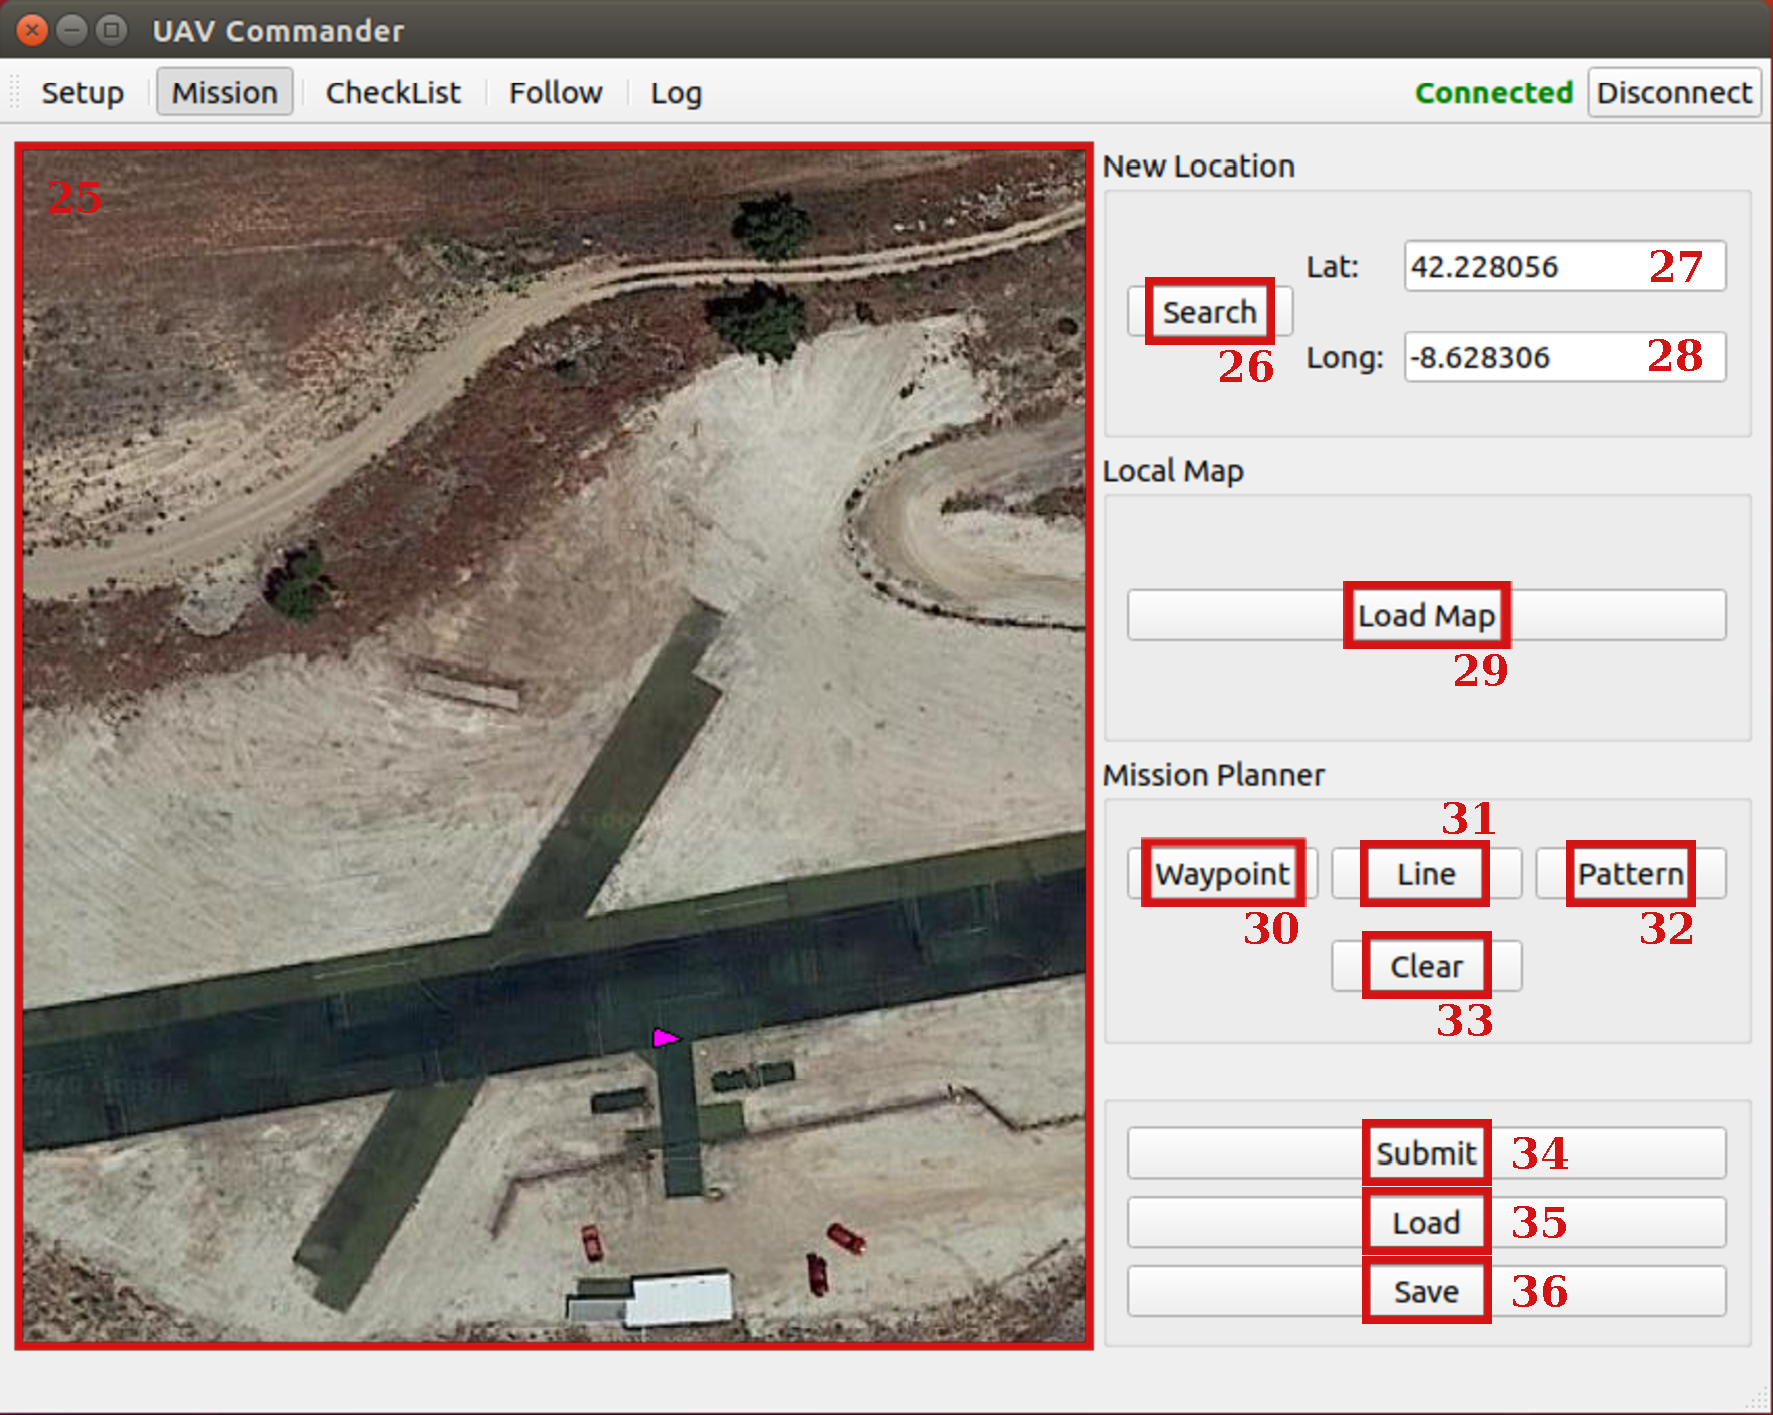
\includegraphics[width=\textwidth]{man/mission.pdf}
\end{figure}

\begin{table}[H]
    \centering
    \begin{threeparttable}
        \begin{tabular}{| l | l |}
            \hline
            \thead{Nº} & \thead{Descripción} \\ \hline
            
            25 & Escena con el mapa cargado. \\ \hline
            26 & Botón para buscar determinada posición en el mapa. \\ \hline
            27 & Latitud (º). \\ \hline
            28 & Longitud (º). \\ \hline
            29 & Botón de carga de mapa local. \\ \hline
            30 & Botón para acceder al creador de misiones multilínea (Ver \ref{subsubsection:app-pol}). \\ \hline
            31 & No disponible. \\ \hline
            32 & Botón para acceder al creador de misiones por patrón (Ver \ref{subsubsection:app-patron}). \\ \hline
            33 & Botón para borrar la misión activa. \\ \hline
            34 & Botón para crear la misión. \\ \hline
            35 & Botón para cargar una misión. \\ \hline
            36 & Botón para guardar la misión. \\ \hline
        \end{tabular}
        
    \end{threeparttable}
\end{table}

\clearpage

\subsubsection{Creador de misiones polilínea} \label{subsubsection:app-pol}

\begin{figure}[H]
    \centering
    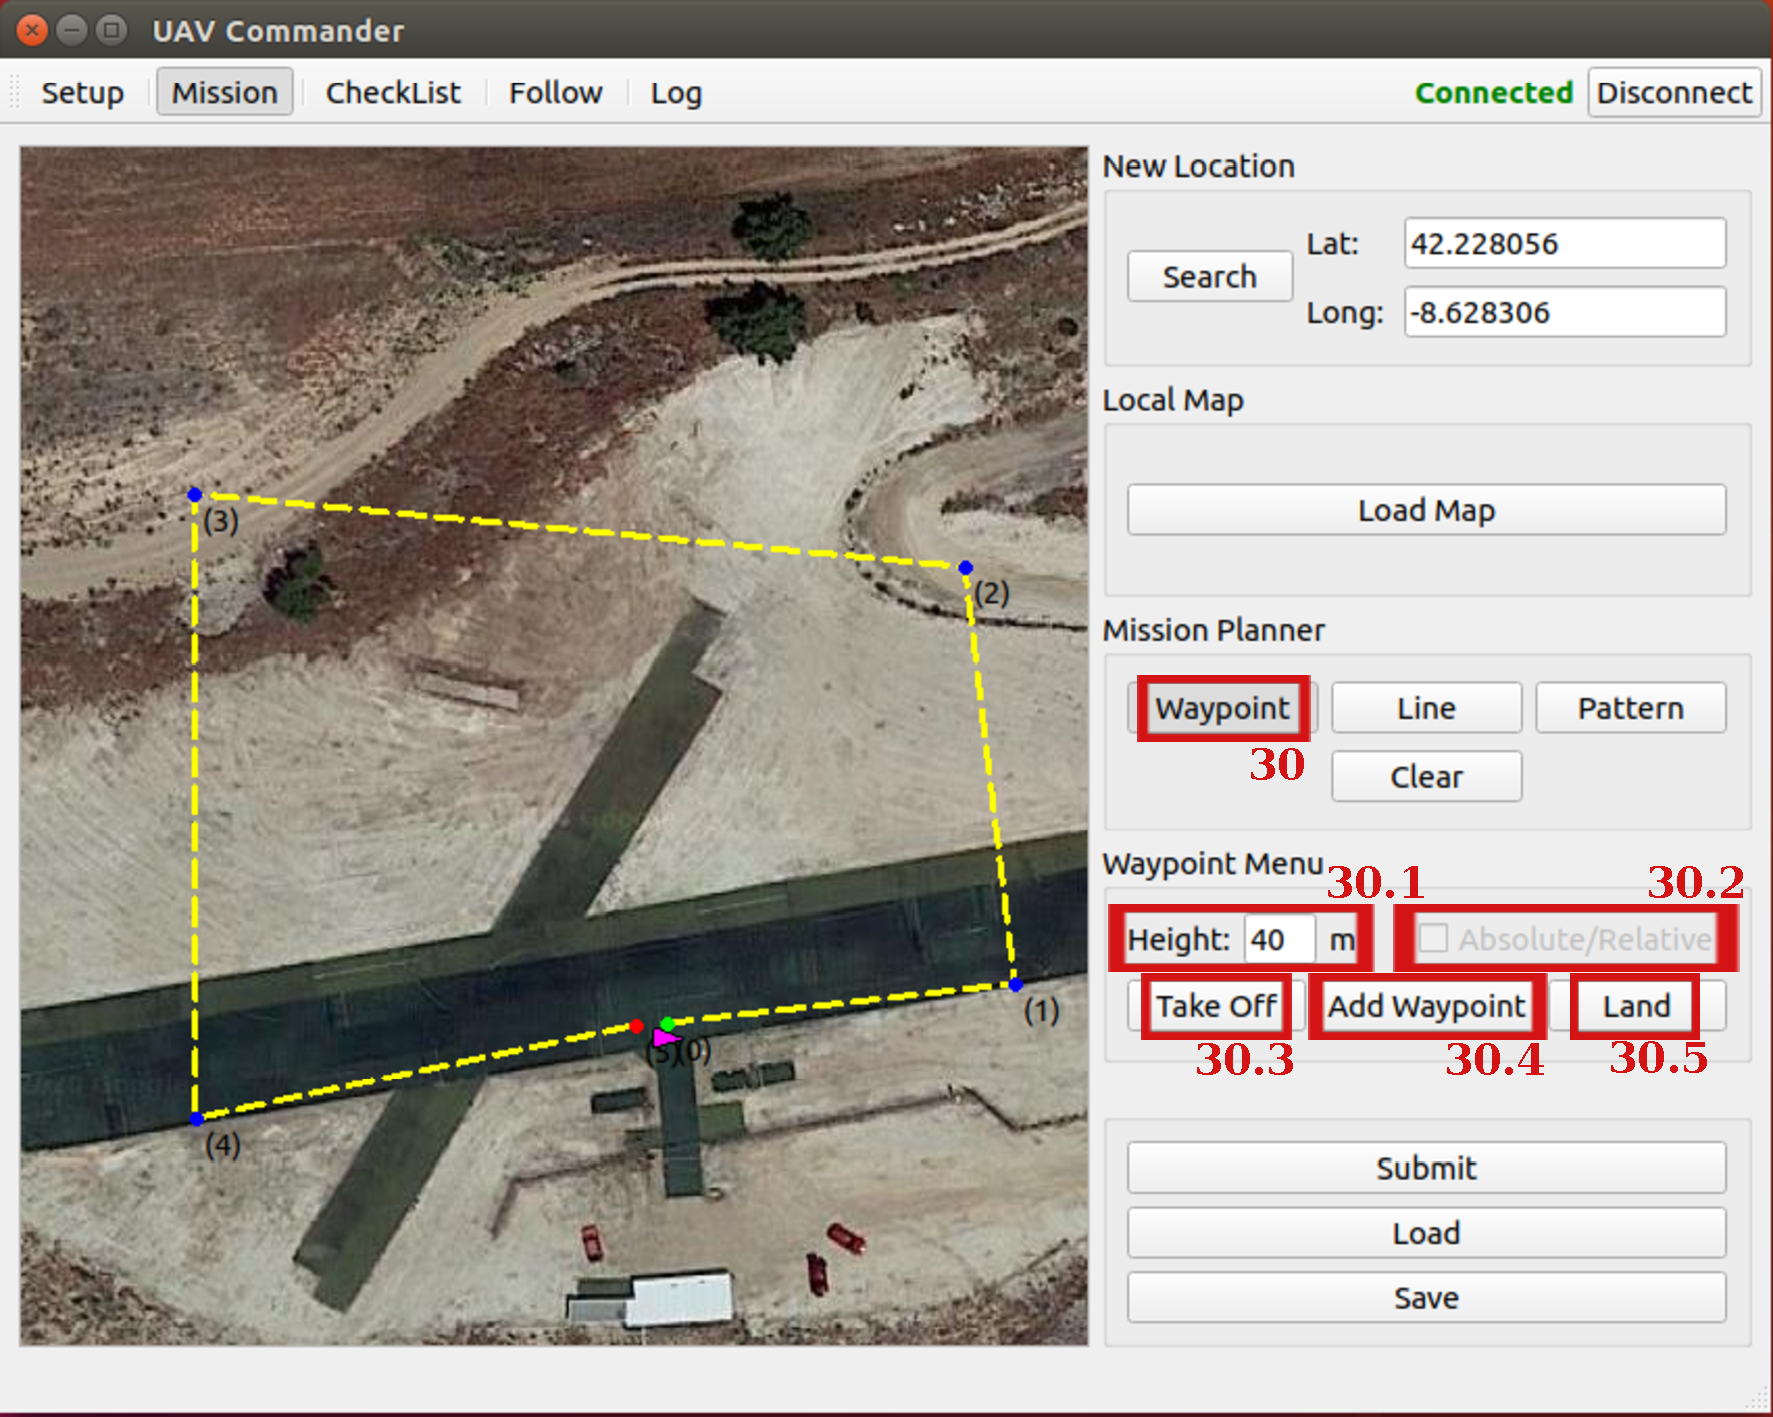
\includegraphics[width=\textwidth]{man/mission-wayp.pdf}
\end{figure}

\begin{table}[H]
    \centering
    \begin{threeparttable}
        \begin{tabular}{| l | l |}
            \hline
            \thead{Nº} & \thead{Descripción} \\ \hline
            
            30.1 & Altura (m). \\ \hline
            30.2 & Altura absoluta o relativa. \\ \hline
            30.3 & Botón para añadir punto de despegue. \\ \hline
            30.4 & Botón para abrir ventana de puntos de paso (Ver \ref{subsection:app-puntos}). \\ \hline
            30.5 & Botón para añadir punto de aterrizaje. \\ \hline
        \end{tabular}
        
    \end{threeparttable}
\end{table}

\clearpage

\subsubsection{Creador de misiones por patrón} \label{subsubsection:app-patron}

\begin{figure}[H]
    \centering
    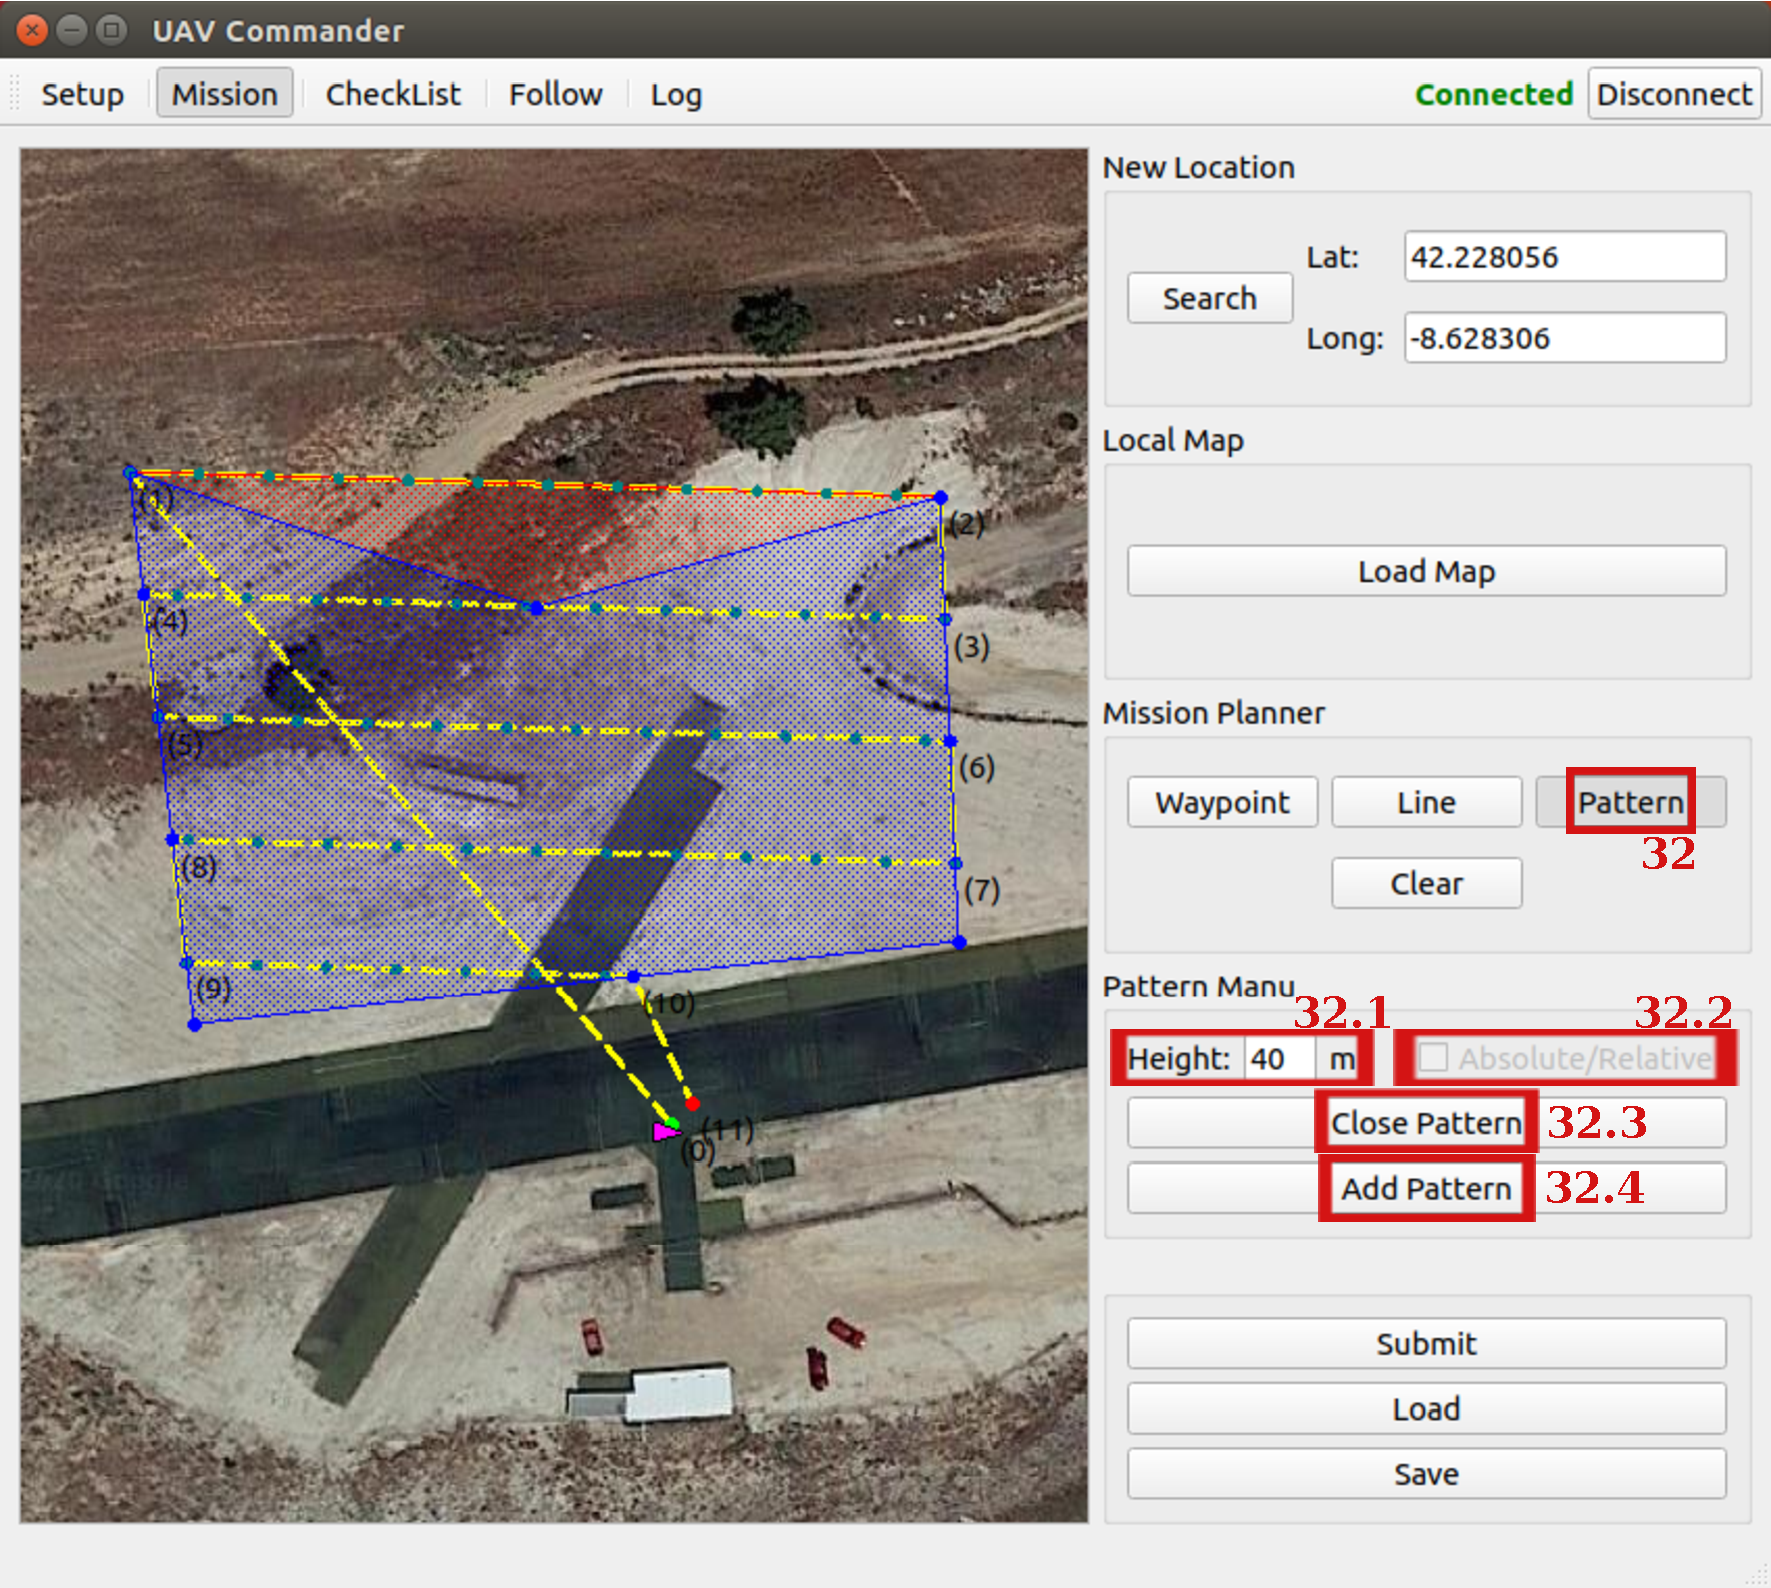
\includegraphics[width=\textwidth]{man/mission-pattern.pdf}
\end{figure}

\begin{table}[H]
    \centering
    \begin{threeparttable}
        \begin{tabular}{| l | l |}
            \hline
            \thead{Nº} & \thead{Descripción} \\ \hline
            
            32.1 & Altura (m). \\ \hline
            32.2 & Altura absoluta o relativa. \\ \hline
            32.3 & Botón para cerrar el patrón. \\ \hline
            32.4 & Botón para abrir ventana de vértices (Ver \ref{subsection:app-puntos}). \\ \hline
        \end{tabular}
        
    \end{threeparttable}
\end{table}

\clearpage

\subsection{Pestaña \emph{Checklist}} \label{subsection:app-check}

\begin{figure}[H]
    \centering
    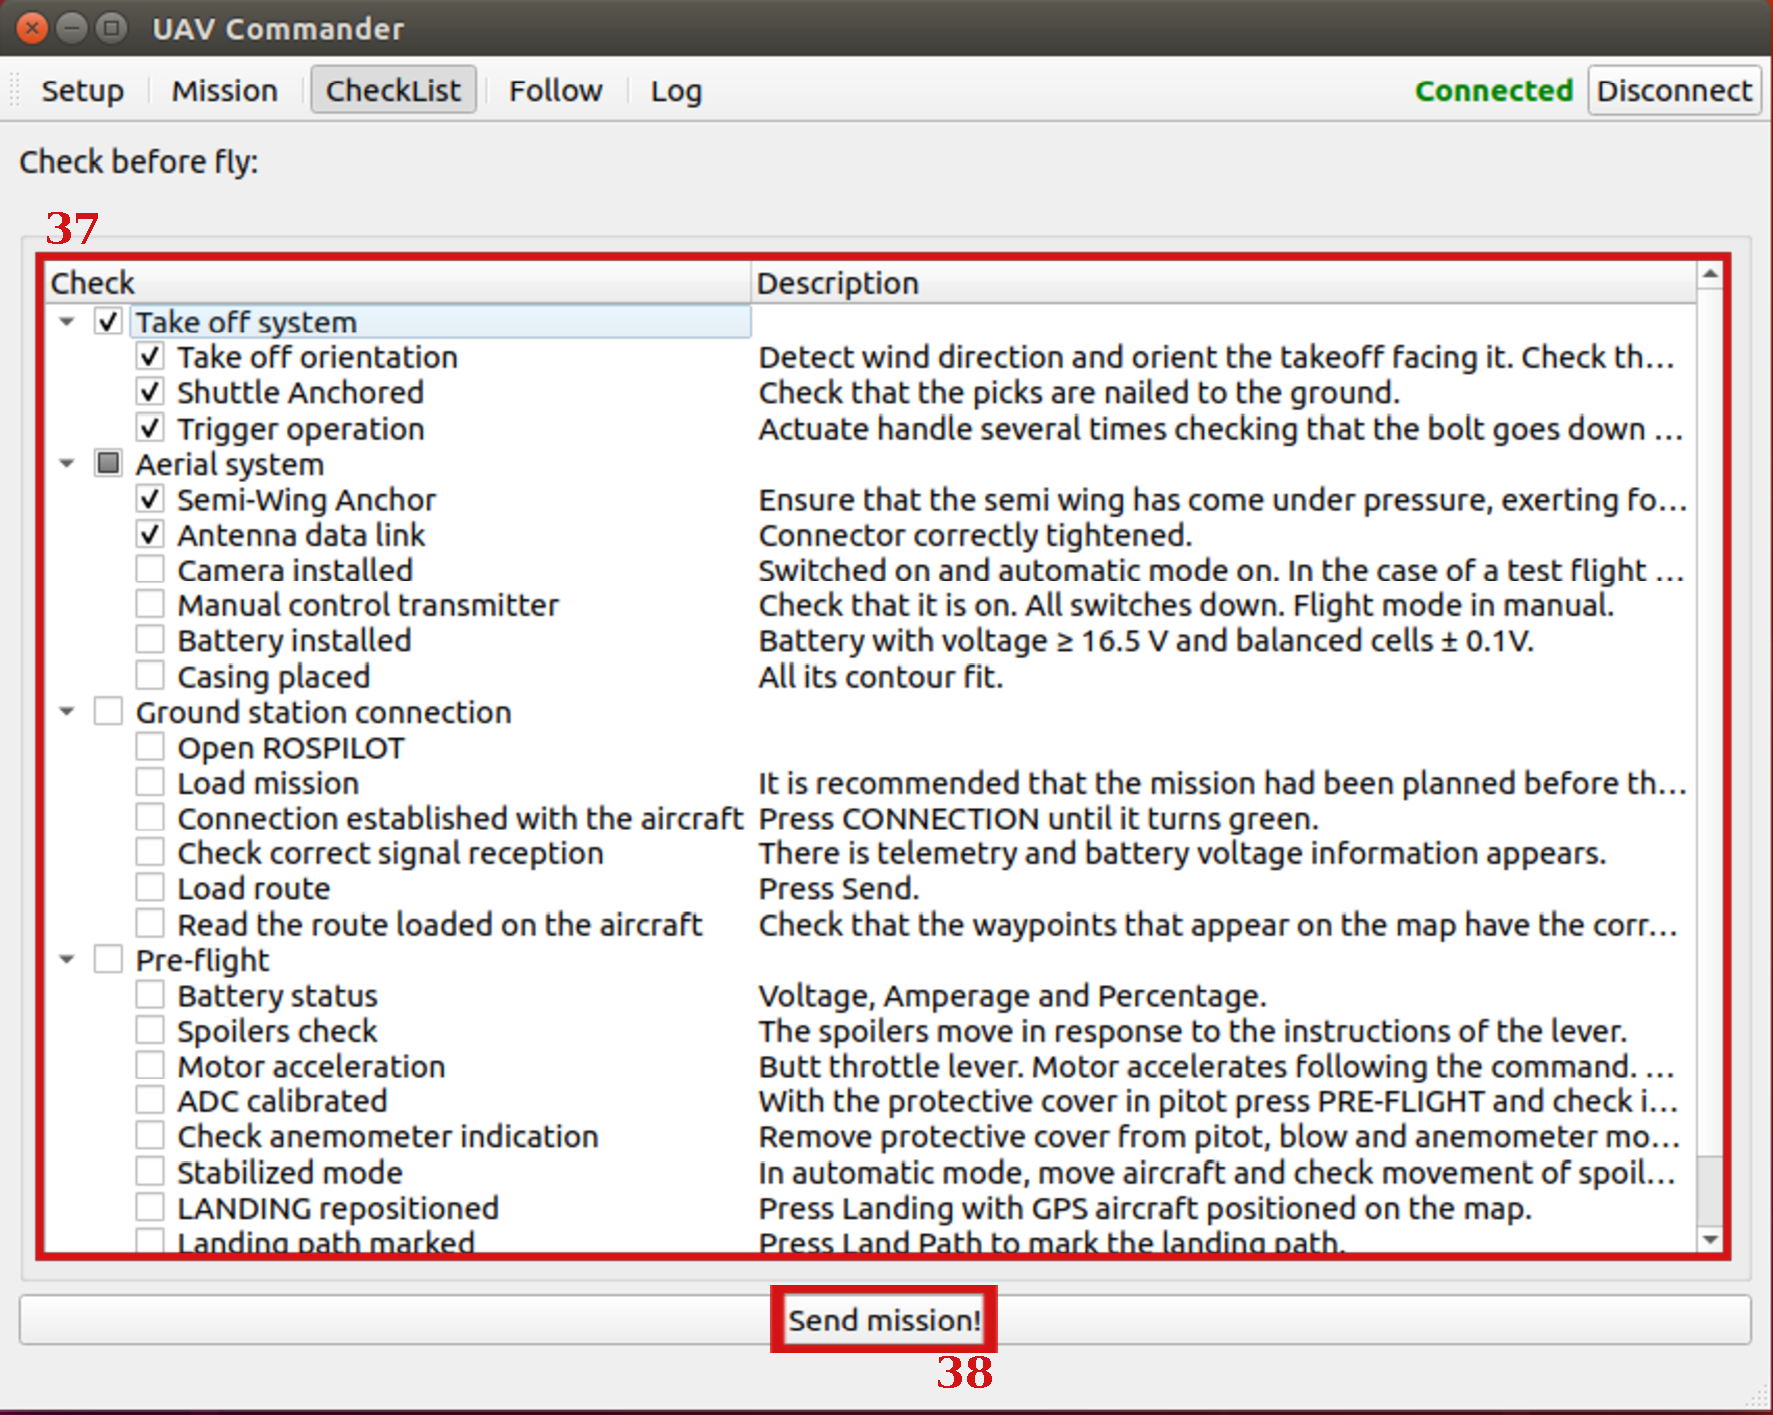
\includegraphics[width=\textwidth]{figures/man/checklist.pdf}
\end{figure}

\begin{table}[H]
    \centering
    \begin{threeparttable}
        \begin{tabular}{| l | l |}
            \hline
            \thead{Nº} & \thead{Descripción} \\ \hline
            
            37 & Listado de comprobaciones pre-vuelo. \\ \hline
            38 & Botón para enviar la misión a la aeronave. \\ \hline
        \end{tabular}
        
    \end{threeparttable}
\end{table}

\clearpage

\subsection{Pestaña \emph{Follow}} \label{subsection:app-follow}

\begin{figure}[H]
    \centering
    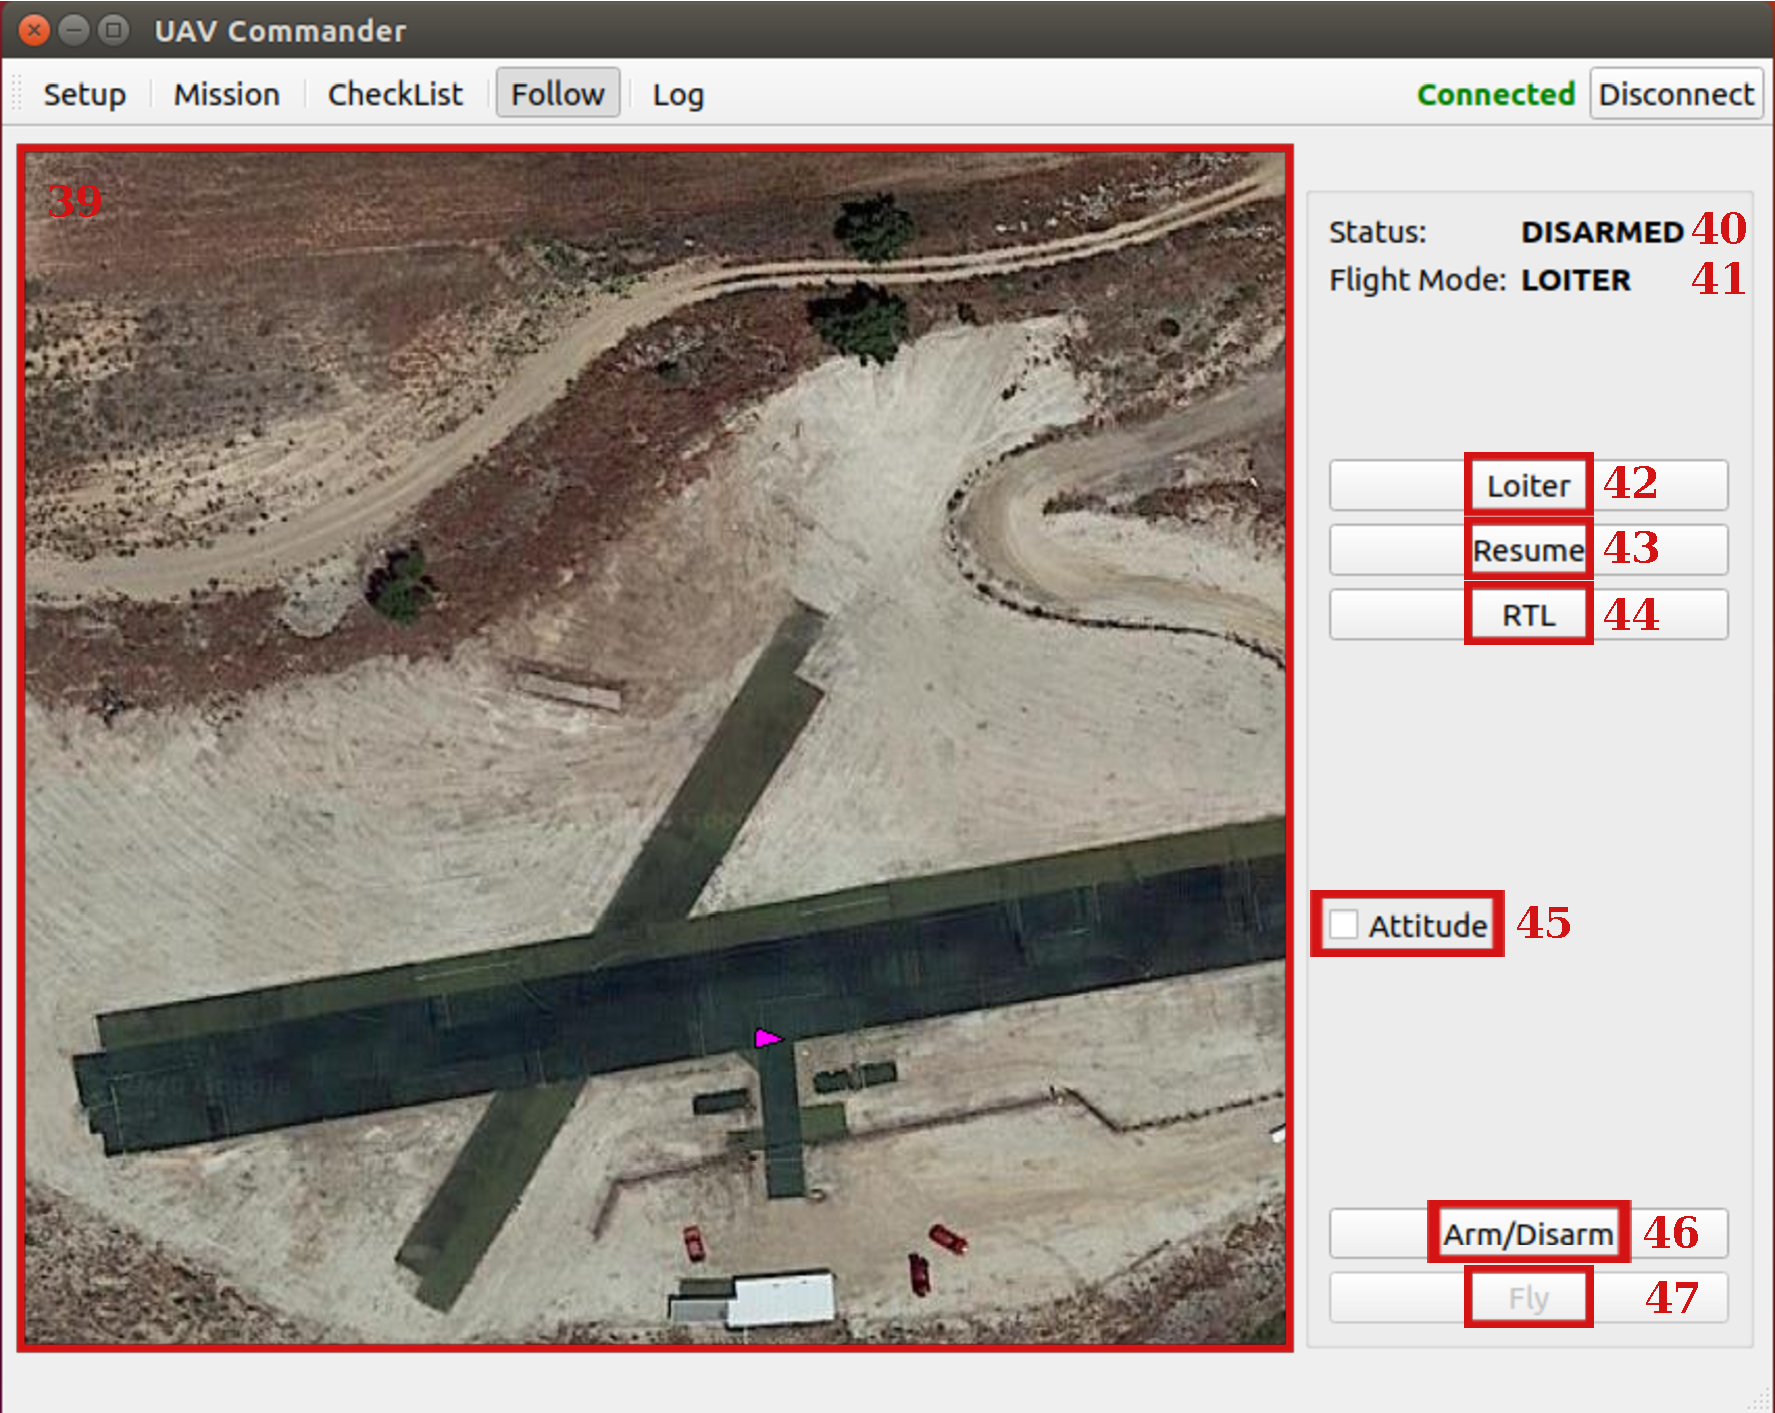
\includegraphics[width=\textwidth]{man/follow.pdf}
\end{figure}

\begin{table}[H]
    \centering
    \begin{threeparttable}
        \begin{tabular}{| l | l |}
            \hline
            \thead{Nº} & \thead{Descripción} \\ \hline
            
            39 & Escena con el mapa cargado. \\ \hline
            40 & Etiqueta que muestra el estado de la aeronave. \\ \hline
            41 & Etiqueta que muestra el modo de vuelo de la aeronave. \\ \hline
            42 & Botón para activar el modo de vuelo \emph{Loiter}. \\ \hline
            43 & Botón para activar el modo de vuelo \emph{Auto}. \\ \hline
            44 & Botón para activar el modo de vuelo \emph{RTL}. \\ \hline
            45 & Botón para abrir la pestaña secundaria de sensores (Ver \ref{subsection:app-sensor}). \\ \hline
            46 & Botón para armar/desarmar. \\ \hline
            47 & Botón para despegar e iniciar misión. \\ \hline
        \end{tabular}
        
    \end{threeparttable}
\end{table}

\clearpage

\subsection{Pestaña \emph{Log}} \label{subsection:app-log}

\begin{figure}[H]
    \centering
    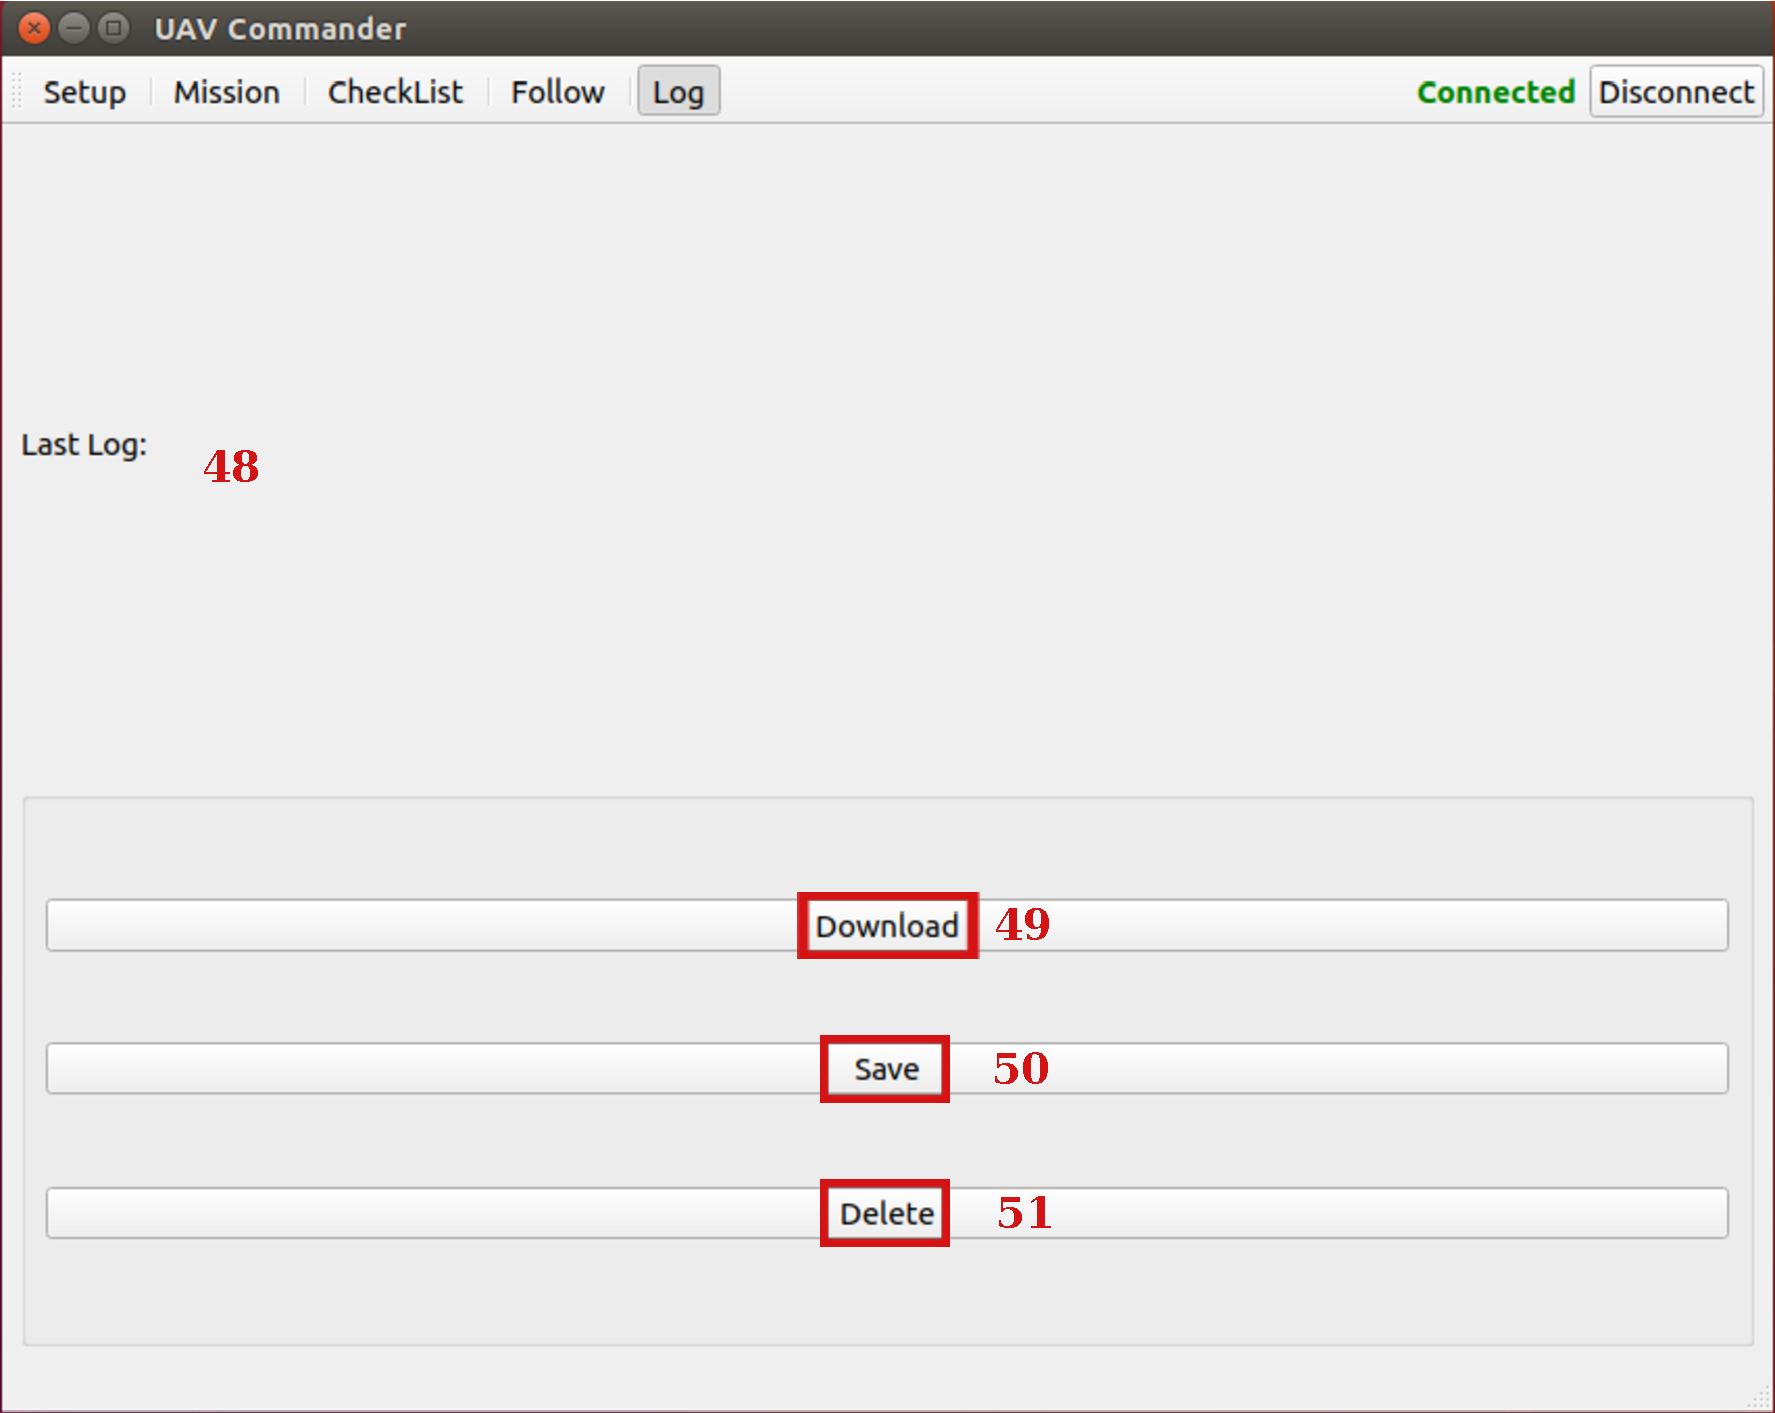
\includegraphics[width=\textwidth]{man/log.pdf}
\end{figure}

\begin{table}[H]
    \centering
    \begin{threeparttable}
        \begin{tabular}{| l | l |}
            \hline
            \thead{Nº} & \thead{Descripción} \\ \hline
            
            48 & Etiqueta que muestra último log descargado. \\ \hline
            49 & Botón para descargar los logs del autopiloto. \\ \hline
            50 & Botón para guardar los logs descargados. \\ \hline
            51 & Botón para borrar los logs del autopiloto. \\ \hline
        \end{tabular}
        
    \end{threeparttable}
\end{table}

\clearpage

\section{Ventanas Secundarias} \label{section:app-vent-sec}

\subsection{Ventana de Configuración} \label{subsection:app-config}

\begin{figure}[H]
    \centering
    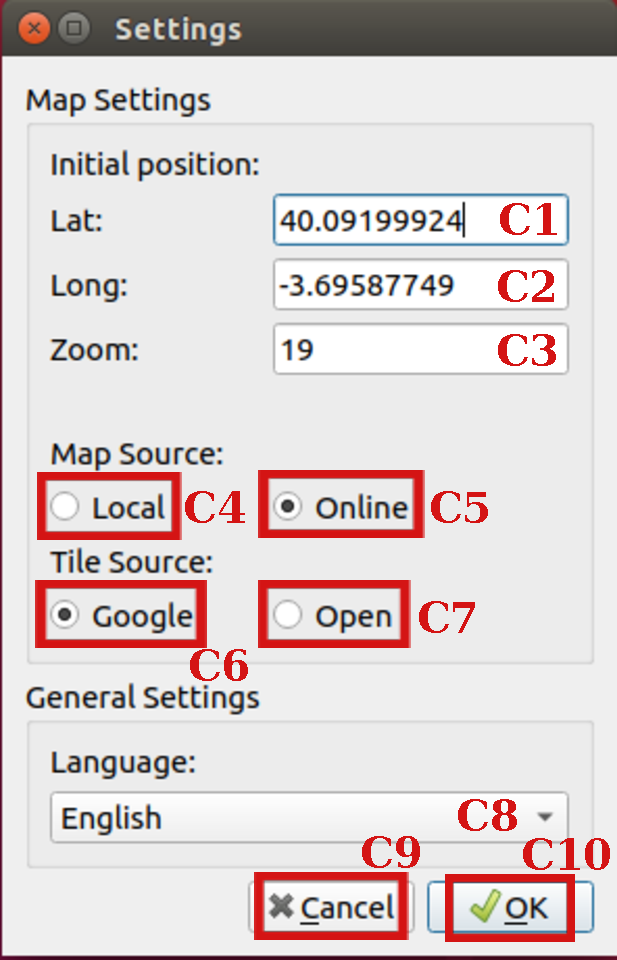
\includegraphics[width=0.4\textwidth]{man/settings.pdf}
\end{figure}

\begin{table}[H]
    \centering
    \begin{threeparttable}
        \begin{tabular}{| l | l |}
            \hline
            \thead{Nº} & \thead{Descripción} \\ \hline
            
            C1  & Latitud por defecto de la escena (º). \\ \hline
            C2  & Longitud por defecto de la escena (º). \\ \hline
            C3  & Zoom por defecto de la escena. \\ \hline
            C4  & Botón para activar mapas locales sobre la escena. \\ \hline
            C5  & Botón para activar mapas en línea sobre la escena. \\ \hline
            C6  & Botón para activar mapas de Google sobre la escena. \\ \hline
            C7  & Botón para activar mapas abiertos sobre la escena. \\ \hline
            C8  & Desplegable para seleccionar el idioma de la interfaz gráfica de usuario. \\ \hline
            C9  & Botón para cancelar cambios. \\ \hline
            C10 & Botón para confirmar cambios. \\ \hline
        \end{tabular}
        
    \end{threeparttable}
\end{table}

\clearpage

\subsection{Ventana de carga de Mapa Local} \label{subsection:app-local}

\begin{figure}[H]
    \centering
    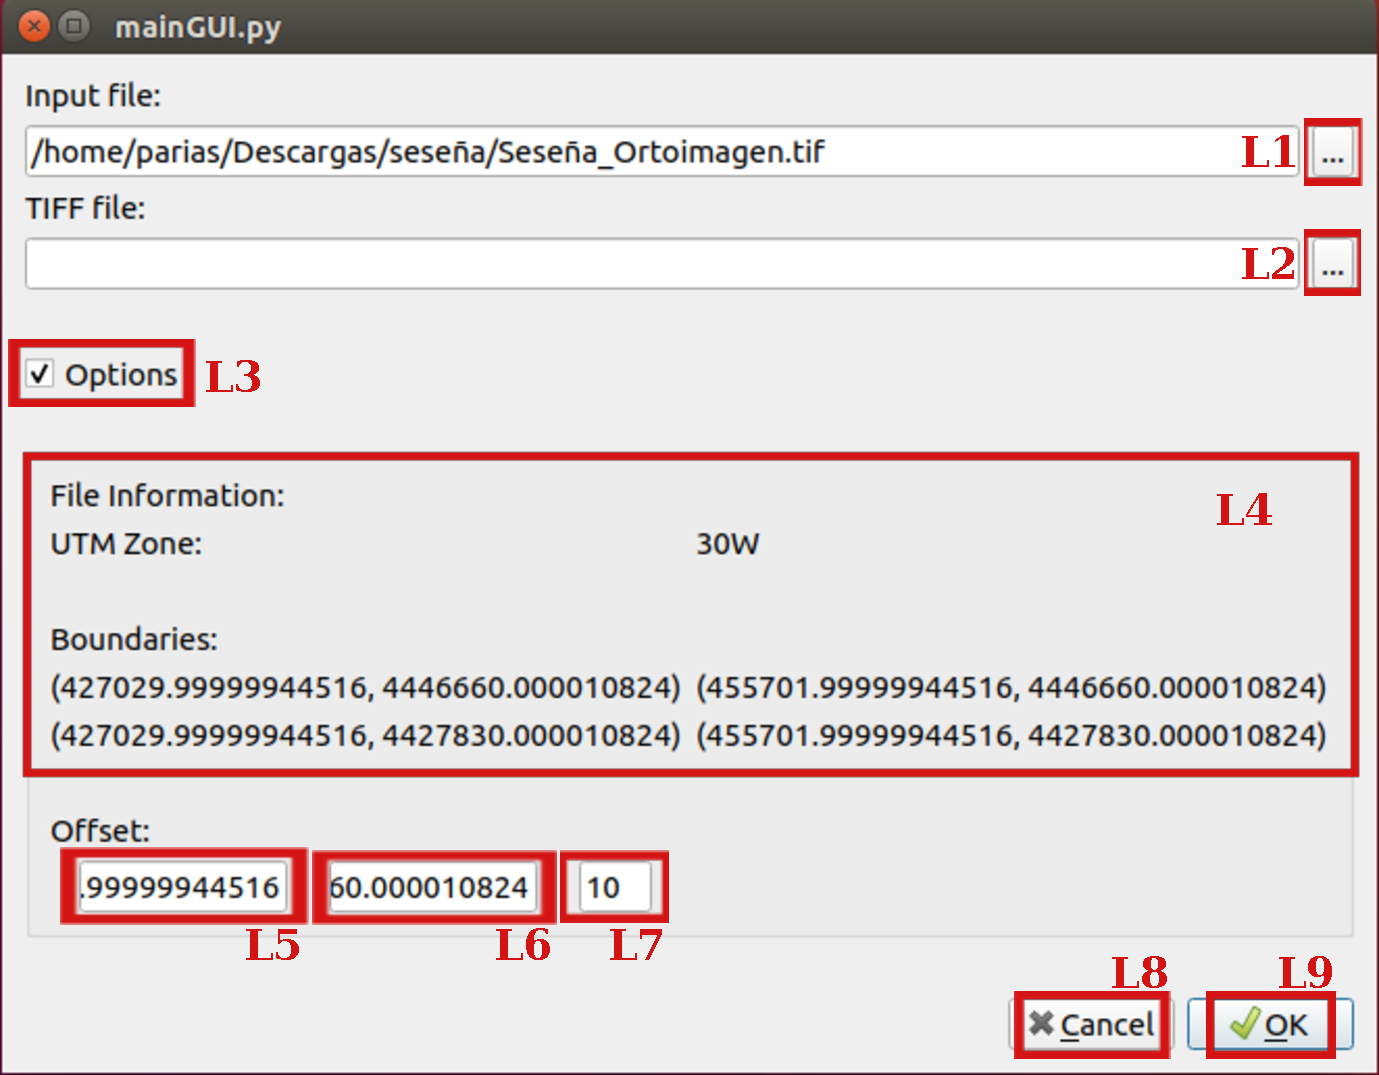
\includegraphics[width=0.8\textwidth]{man/local_map.pdf}
\end{figure}

\begin{table}[H]
    \centering
    \begin{threeparttable}
        \begin{tabular}{| l | l |}
            \hline
            \thead{Nº} & \thead{Descripción} \\ \hline
            
            L1 & Botón para cargar archivo con ortoimagen. \\ \hline
            L2 & Botón para cargar archivo con elevaciones. \\ \hline
            L3 & Botón para ostrar/ocultar opciones. \\ \hline
            L4 & Información sobre ortoimagen cargada. \\ \hline
            L5 & Coordenada X (UTM) a cargar (m). \\ \hline
            L6 & Coordenada Y (UTM) a cargar (m). \\ \hline
            L7 & Zoom a cargar. \\ \hline
            L8 & Botón para cancelar cambios. \\ \hline
            L9 & Botón para confirmar cambios. \\ \hline
        \end{tabular}
        
    \end{threeparttable}
\end{table}

\clearpage

\subsection{Ventana de Puntos de Paso} \label{subsection:app-puntos}

\begin{figure}[H]
    \centering
    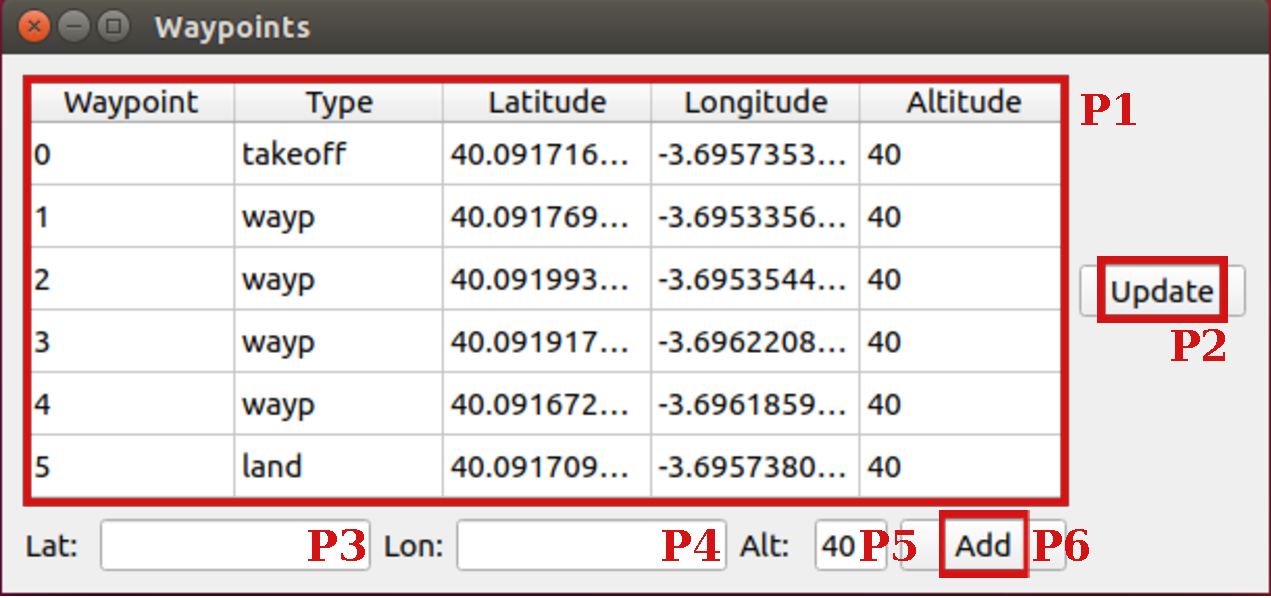
\includegraphics[width=0.8\textwidth]{man/wayp_window.pdf}
\end{figure}

\begin{table}[H]
    \centering
    \begin{threeparttable}
        \begin{tabular}{| l | l |}
            \hline
            \thead{Nº} & \thead{Descripción} \\ \hline
            
            P1 & Lista con los puntos de paso de la misión. \\ \hline
            P2 & Botón para actualizar los puntos de la lista sobre la escena. \\ \hline
            P3 & Latitud (º). \\ \hline
            P4 & Longitud (º). \\ \hline
            P5 & Altura (m). \\ \hline
            P6 & Botón para añadir un punto de paso a la lista. \\ \hline
        \end{tabular}
        
    \end{threeparttable}
\end{table}

\clearpage

\subsection{Ventana de Sensores} \label{subsection:app-sensor}

\begin{figure}[H]
    \centering
    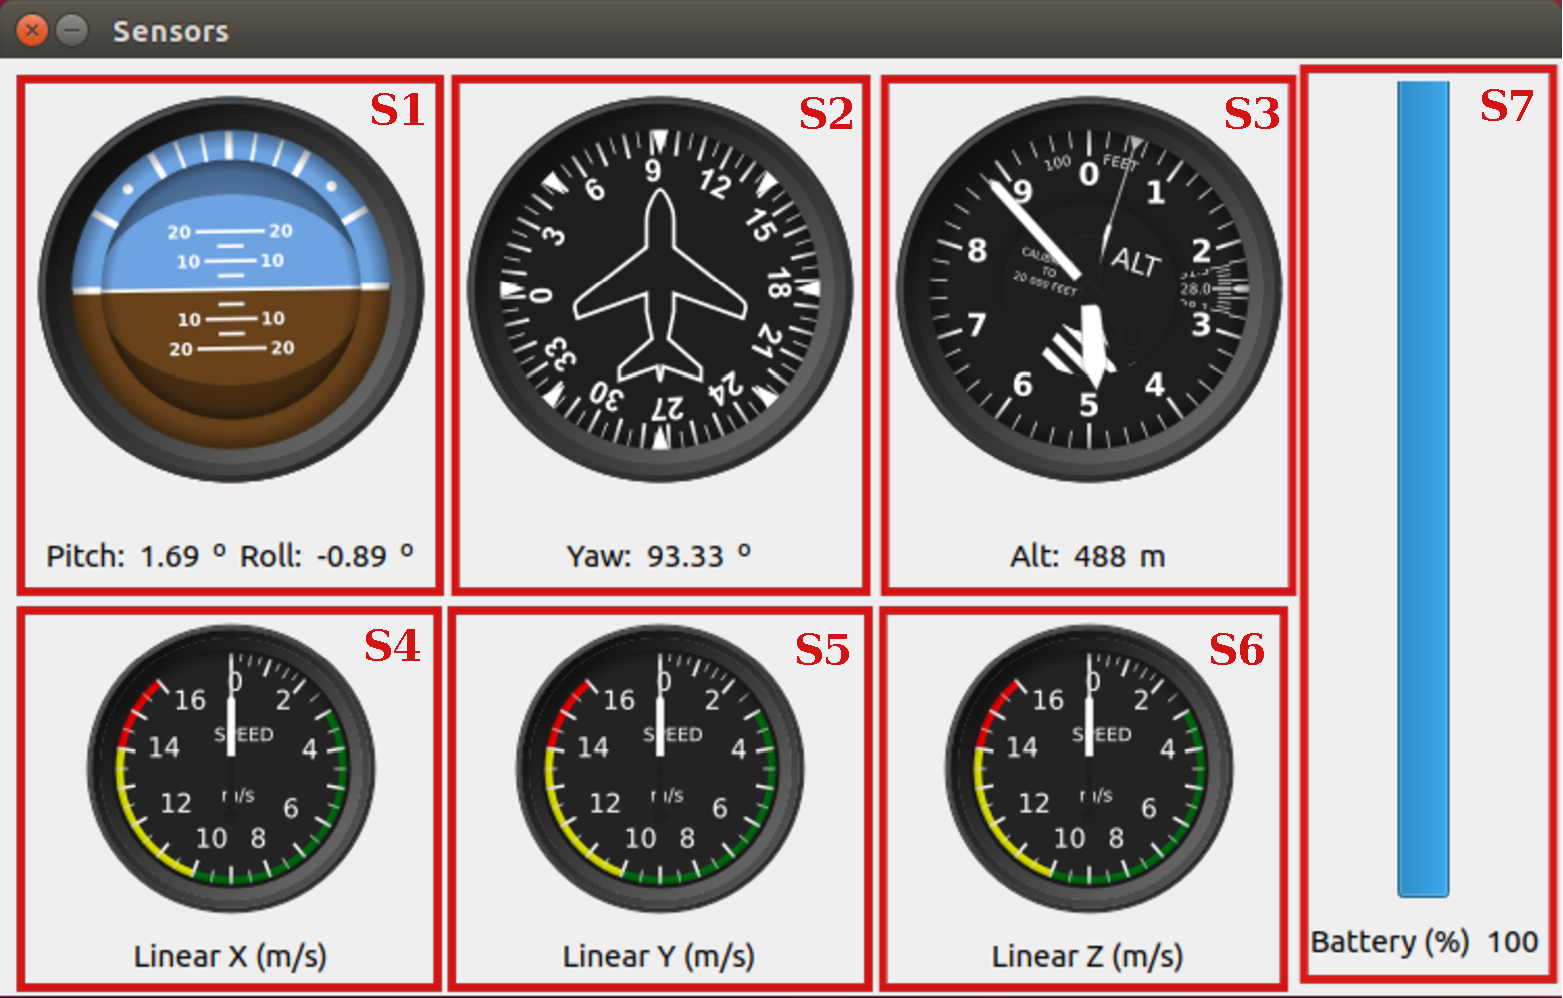
\includegraphics[width=\textwidth]{man/sensors.pdf}
\end{figure}

\begin{table}[H]
    \centering
    \begin{threeparttable}
        \begin{tabular}{| l | l |}
            \hline
            \thead{Nº} & \thead{Descripción} \\ \hline
            
            S1 & Horizonte artificial. \\ \hline
            S2 & Indicador de rumbo. \\ \hline
            S3 & Altímetro. \\ \hline
            S4 & Velocidad lineal X. \\ \hline
            S5 & Velocidad lineal Y. \\ \hline
            S6 & Velocidad lineal Z. \\ \hline
            S7 & Batería. \\ \hline
        \end{tabular}
        
    \end{threeparttable}
\end{table}

\clearpage